\section{Unikonzert SS 2022}
\sectionmark{Unikonzert SS 2022}


\begin{figure}[h]
    \centering 
    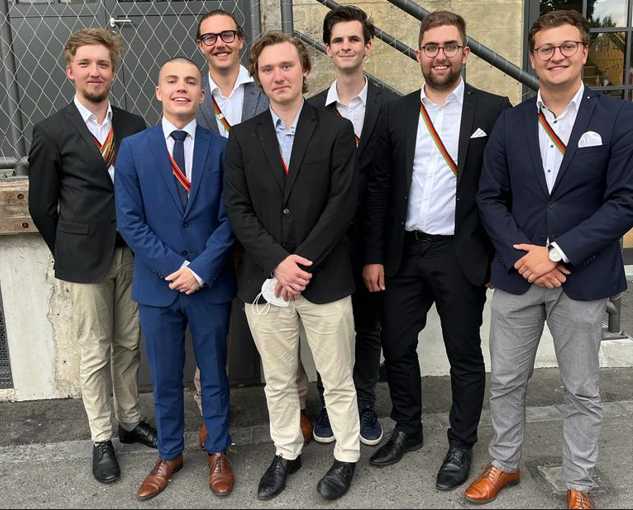
\includegraphics[width=0.8\textwidth]{./Bilder/1.0_unikonzert/1.unikonzert.png}
    \caption{}
\end{figure}

\begin{multicols}{2}	
Als musikalischer Höhepunkt des Semesterprogramms war am Montag, dem 04.07.2022 der gemeinsame Besuch des Uni-Konzerts der Münchner Philharmoniker geplant. Wie der Name der Veranstaltung bereits impliziert, war die Teilnahme am Konzert nur Studenten und jeweils einer Begleitperson gestattet, die Eintrittspreise für diese Veranstaltung gestalteten sich aus diesem Grund auch sehr studentenfreundlich.
Zu acht ging es also los Richtung Isarphilharmonie im Gasteig HP8, wo uns der musikalische Hochgenuss erwarten sollte. 

Abweichend vom ursprünglichen Programm, das aufgrund familiärer Gründe eines Solisten kurzfristig geändert werden musste, spielte das Orchester im ersten Teil des Abends das Konzert für Violine und Orchester Nr. 1 a-Moll op.77 von Dimitrij Schostakowitsch. Dieses 1948 in der Sowjetunion komponierte Violinkonzert musste der Komponist nach Fertigstellung aufgrund der strengen Kulturdoktrin der Stalin Zeit vorerst bewusst zurückhalten. Es enthält neben damals unerwünschten harmonischen und thematischen Strukturen auch einen Teil, der einigen jüdischen Volksliedern nahesteht und hätte schon aus diesem Grund in der Sowjetunion der Stalin Zeit keine Chance gehabt. Die Bundesbrüder inklusive mir imponierte vor allem die Fähigkeiten der Solistin an der Violine.

Nach einer kurzen Pause ging es mit einem etwas moderneren Stück weiter. John Adams "The Chairman Dances" (der Vorsitzende tanzt) entstammt der Oper "Nixon in China", in der Präsident Nixon 1972 als erster amerikanischer Präsident die Volksrepublik China besucht und dabei auf Mao Zedong trifft. Vor allem das Foxtrott Thema des letzten Aktes, zu dem das Staatsoberhaupt der Volksrepublik mit seiner Ehefrau in der Oper tanzt, fand großen Anklang im Publikum. 

Der dritte Teil des Abends bestand aus symphonischen Tänzen des Musicals "West Side Story", das mit seiner Uraufführung 1957 die Musical Szene des New Yorker Broadways revolutionierte und seinen Komponisten Leonard Bernstein zu einem der wichtigsten Bühnenkomponisten unserer Zeit machte. 

Im Anschluss an das Konzert fand noch ein musikalisch begleiteter Ausklang in der Vorhalle des Konzertsaals statt, der aber, vermutlich aufgrund der nicht gerade studentenfreundlichen Getränkepreise, nicht sonderlich attraktiv erschien.


	%
	\begin{flushright}
		\hfill\emph{Felix Fiesel Va!}
	\end{flushright}
	%	
\end{multicols}
%


\begin{figure}
	\center
	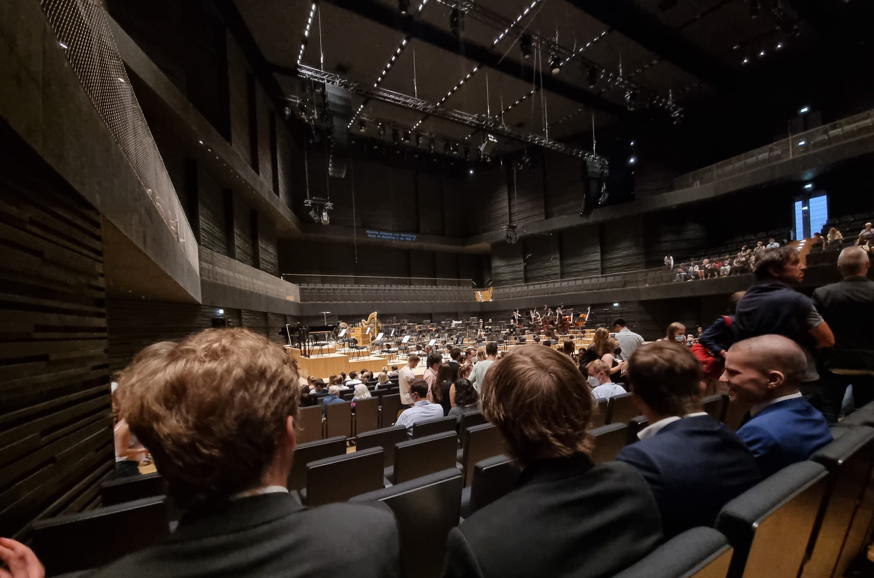
\includegraphics[width=0.8\linewidth]{./Bilder/1.0_unikonzert/3.voller_Saal.png} 
    
    \caption{}
\end{figure}